\subsection{Precision Discussion of \widening}

\begin{figure}[tp]
    \hfill
    \begin{subfigure}[b]{.22\textwidth}
        \centering
        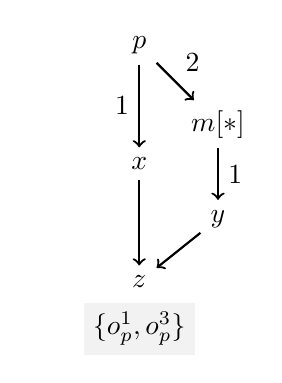
\begin{tikzpicture}[scale=1,thick]
    \node (p) at (0, 0) {$\textpurple{p}$};
    \node (x) at (0, -1.5) {$x$};
    \node (m) at (1, -1) {$m[*]$};
    \node (y) at (1, -2.2) {$y$};
    \node (z) at (0, -3) {$z$};

    \draw [->] (p) --node[left]{$1$} (x);
    \draw [->] (x) -- (z);
    \draw [->] (p) --node[above right]{$2$} (m);
    \draw [->] (m) --node[right]{$1$} (y);
    \draw [->] (y) -- (z);

    \node at (-1.3, 0) {};

    \node[fill=gray!10] (t) at (0, -3.6) {$\{o_p^1, o_p^3\}$};
\end{tikzpicture}

        \caption{Acyclic Pattern.}\label{fig:acyclic-pattern}
    \end{subfigure}
    \hfill
    \begin{subfigure}[b]{.31\textwidth}
        \centering
        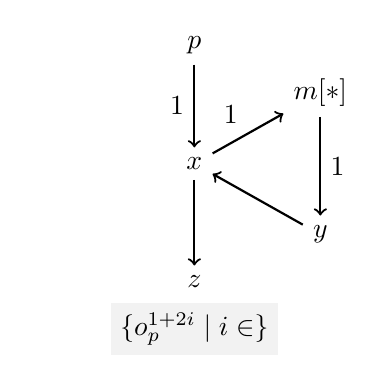
\begin{tikzpicture}[scale=1,thick]
    \node (p) at (0, 0) {$\textpurple{p}$};
    \node (x) at (0, -1.5) {$x$};
    \node (m) at (1.6, -0.6) {$m[*]$};
    \node (y) at (1.6, -2.4) {$y$};
    \node (z) at (0, -3) {$z$};
    \node[fill=gray!10] at (0, -3.6) {$\{o_p^{1 + 2i} \mid  i \in \nats\}$};

    \draw [->] (p) --node[left]{$1$} (x);
    \draw [->] (x) --node[above left]{$1$} (m);
    \draw [->] (m) --node[right]{$1$} (y);
    \draw [->] (y) -- (x);
    \draw [->] (x) -- (z);

    \node at (-2, 0) {};
\end{tikzpicture}

        \caption{Single-Cycle Pattern.}\label{fig:single-cycle-pattern}
    \end{subfigure}
    \hfill
    \hfill
    \begin{subfigure}[b]{.32\textwidth}
        \centering
        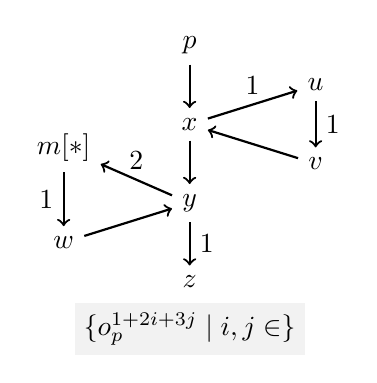
\begin{tikzpicture}[scale=1,thick]
    \node (p) at (0, 0) {$\textpurple{p}$};
    \node (x) at (0, -1) {$x$};
    \node (u) at (1.6, -0.5) {$u$};
    \node (v) at (1.6, -1.5) {$v$};
    \node (y) at (0, -2) {$y$};
    \node (m) at (-1.6, -1.3) {$m[*]$};
    \node (w) at (-1.6, -2.5) {$w$};



    \node (z) at (0, -3) {$z$};
    \node[fill=gray!10] at (0, -3.6) {$\{o_p^{1 + 2i + 3j} \mid  i, j \in \nats\}$};

    \draw [->] (p) -- (x);
    \draw [->] (x) --node[above]{$1$} (u);
    \draw [->] (u) --node[right]{$1$} (v);
    \draw [->] (v) -- (x);
    \draw [->] (x) -- (y);
    \draw [->] (y) --node[above]{$2$} (m);
    \draw [->] (m) --node[left]{$1$} (w);
    \draw [->] (w) -- (y);
    \draw [->] (y) --node[right]{$1$} (z);
\end{tikzpicture}

        \caption{Multiple-Cycle Pattern.}\label{fig:multiple-cycles-pattern}
    \end{subfigure}
    \hfill
    \caption{
        Representative TIG patterns for discussing the precision of \widening, focusing on $\absT(z)$ for simplicity.
        The ideal \tia results without \widening are shown in gray boxes.
    }\label{fig:precision-pattern}.
\end{figure}

In this section, we discuss the precision trade-off introduced by $\widening$ to ensure convergence.
For simplicity, we focus on the temporal influence objects associated with a single input port $p$, since $\widening$ processes each port independently (Line~\ref{line:port} of Algorithm~\ref{alg:widening}).
Figure~\ref{fig:precision-pattern} illustrates three representative TIG patterns and their corresponding ideal \tia results without \widening.
We next examine how applying $\widening$ affects the precision of \tia for each pattern.

\paragraph{Acyclic Pattern}

As illustrated in Figure~\ref{fig:acyclic-pattern}, when all paths in the TIG from input port $p$ to location $z$ are acyclic, $\absT(z)$ is finite.
Therefore, if the widening threshold is sufficiently large such that $N > |\absT(z)|$, $\widening$ is never triggered for $\absT(z)$, and $\widening(\absT(z)) = \absT(z)$ by Line~\ref{line:threshold} of Algorithm~\ref{alg:widening}.
Thus, widening introduces no precision loss in this case.
Theoretically, such an $N$ always exists because $\absT(z)$ is finite.
However, determining the smallest such threshold in general would require computing the precise temporal influence information, which is precisely the information that the analysis is intended to approximate.
In practice, we therefore choose a sufficiently large fixed threshold rather than computing a circuit-specific threshold.

Moreover, the number of distinct propagation delays along acyclic TIG paths between two circuit locations is typically expected to remain relatively small in synchronous hardware designs.
For example, the two incoming TIG edges to $z$ in Figure~\ref{fig:acyclic-pattern} can only arise from a wire connection such as $z = x \mathbin{\vop} y$ (where $\vop$ is an operator) through rule~\rTiaWire.
In typical designs, the operands of such expressions combine a limited number of paths with different pipeline depths, rather than intentionally combining a large number of distinct propagation delays.
Thus, when $\absT(z)$ is finite, its cardinality is generally expected to remain manageable for a reasonably large widening threshold.

\paragraph{Single Cycles Pattern}

As illustrated in Figure~\ref{fig:single-cycle-pattern}, suppose that all paths from $p$ to $z$ contain at most one cycle, and that the cycle has propagation delay $d$.
Traversing the cycle an arbitrary number of times produces temporal influence objects whose delays form an arithmetic progression.
In particular, for some minimum delay $a$, $\absT(z) = \{o_p^{a + di} \mid i \in \nats\}$.
Consequently, when widening is triggered, Lines~\ref{line:init}--\ref{line:widened} of Algorithm~\ref{alg:widening} recover exactly the same arithmetic progression.
For the example in Figure~\ref{fig:single-cycle-pattern},
\[
\begin{aligned}
    \widening(\absT(z)) & = \widening(\{o_p^{1+2i} \mid i\in \nats\})\\
    & = \widening(\{o_p^1, o_p^3, o_p^5, \dots\}) = \{o_p^{1+2i} \mid i \in \nats\} = \absT(z).\\
\end{aligned}
\]
So, widening introduces no precision loss for this pattern either.

\paragraph{Multiple Cycles Pattern}

The precision behavior becomes more interesting when multiple cycles with different propagation delays occur along TIG paths from $p$ to $z$, as illustrated in Figure~\ref{fig:multiple-cycles-pattern}.
In this case, temporal influences can traverse each cycle an arbitrary number of times, and the resulting temporal influence set is generally not itself an arithmetic progression.
For the example in Figure~\ref{fig:multiple-cycles-pattern}, the path contains cycles with propagation delays $2$ and $3$, and the acyclic portion of the path contributes a minimum delay of $1$.
By rule $\rTiaPropa$, the resulting temporal influence set is
\[
\absT(z)=\{o_p^{1+2i+3j}\mid i,j\in\nats\}.
\]
Thus by Line~\ref{line:init}--\ref{line:widened} of Algorithm~\ref{alg:widening} we have:
\[
\begin{aligned}
    \widening(\absT(z)) & = \widening(\{o_p^{1+2i+3j} \mid i, j\in \nats\})\\
    & = \widening(\{o_p^1, o_p^3, o_p^4, o_p^5, o_p^6 \dots\}) = \{o_p^{1+i} \mid i \in \nats\}.\\
\end{aligned}
\]
Hence, in this example, widening introduces only one false positive, namely $o_p^2$:
\[
\widening(\absT(z))-\absT(z)=\{o_p^2\}.
\]
This observation generalizes to arbitrary multiple-cycle patterns.
In such patterns, the temporal influence propagation delays generated by a finite collection of cycles can be expressed as additive combinations of their cycle delays, offset by the minimum delay along a path that traverses none of the cycles.
The following lemma shows that, although $\widening$ may introduce false positives for such infinite sets, it introduces only finitely many of them.

\begin{lemma}[Finite Precision Loss of \widening for Multiple-Cycle Patterns]\label{lem:finite-widening}
    Given a minimum propagation delay $a_0 \in \nats$ and repeatable cycle delays $0 < a_1 < a_2 < \dots < a_n \in \nats$ with $n > 1$, for $p \in \ports$, let
    \[
    O_p = \left\{ o_p^k \mid  \exists i_1,\dots,i_n \in \nats.\ k = a_0 + \sum_{r=1}^{n} a_r i_r \right\}.
    \]
    Then $\widening(O_p) - O_p$ is finite.
\end{lemma}
\begin{proof}
    Let $g = \gcd(a_1,\dots,a_n)$.
    Since $a_0 \in O_p$ and $a_0+a_r \in O_p$ for every $1 \le r \le n$, the common difference computed by $\widening$ (Line~\ref{line:diff} of Algorithm~\ref{alg:widening}) is exactly $g$.
    Moreover, $a_0$ is the minimum element of $O_p$.
    Therefore,
    \[
    \widening(O_p) = \{ o_p^{a_0+gi} \mid i\in\nats \}.
    \]
    Let $b_r=a_r/g$ for $1\le r\le n$.
    Then $\gcd(b_1,\dots,b_n)=1$.
    Consider the additive monoid generated by $b_1,\dots,b_n$:
    \[
    M = \left\{ \sum_{r=1}^{n} b_r i_r \mid i_1,\dots,i_n\in\nats \right\}.
    \]
    Since the generators have greatest common divisor $1$, $M$ is a numerical semigroup and is cofinite in $\nats$~\cite{rosales_numerical_2009};
    that is, there exists some $B\in\nats$ such that every $i\ge B$ belongs to $M$.
    Thus,
    \[
    \forall i \ge B.\ \exists i_1,\dots,i_n\in\nats.\ a_0+gi = a_0+g\sum_{r=1}^{n}b_r i_r = a_0+g\sum_{r=1}^{n}\frac{a_r}{g}\cdot i_r = a_0+\sum_{r=1}^{n}a_r i_r,
    \]
    which implies
    \[
    \forall i \ge B.\ o_p^{a_0+gi}\in O_p.
    \]
    Therefore, all but finitely many elements of $\widening(O_p)$ already belong to $O_p$.
    In particular,
    \[
    \widening(O_p) - O_p \subseteq \{ o_p^{a_0+gi} \mid 0\le i<B \},
    \]
    which is finite.
\end{proof}

\paragraph{Summary}
The three patterns discussed above illustrate the precision behavior of $\widening$.
For acyclic patterns, $\widening$ introduces no precision loss provided that the widening threshold exceeds the finite number of distinct temporal influence objects.
For single-cycle patterns, the temporal influence set is already an arithmetic progression, so $\widening$ is exact and preserves precision.
For multiple-cycle patterns, $\widening$ may introduce false positives, but Lemma~\ref{lem:finite-widening} shows that only finitely many false positives can be introduced.
